% This file was converted to LaTeX by Writer2LaTeX ver. 1.0.2
% see http://writer2latex.sourceforge.net for more info
\documentclass{article}
\usepackage[latin1]{inputenc}
\usepackage[T1]{fontenc}
\usepackage[english]{babel}
\usepackage{amsmath}
\usepackage{amssymb,amsfonts,textcomp}
\usepackage{array}
\usepackage{supertabular}
\usepackage{hhline}
\usepackage[pdftex]{graphicx}
\makeatletter
\newcommand\arraybslash{\let\\\@arraycr}
\makeatother
\setlength\tabcolsep{1mm}
\renewcommand\arraystretch{1.3}
\title{Lingkungan St. Petrus}
\begin{document}
\section[\ \ \ \ \ \ \ \ Sejarah singkat Lingkungan St.
Petrus]{\ \ \ \ \ \ \ \ Sejarah singkat Lingkungan St. Petrus}
\begin{figure}
\centering
 [Warning: Image ignored] % Unhandled or unsupported graphics:
%\includegraphics[width=1.772cm,height=1.93cm]{}

\end{figure}
\begin{figure}
\centering
 [Warning: Image ignored] % Unhandled or unsupported graphics:
%\includegraphics[width=1.243cm,height=1.454cm]{}

\end{figure}
\begin{figure}
\centering
 [Warning: Image ignored] % Unhandled or unsupported graphics:
%\includegraphics[width=1.56cm,height=1.772cm]{}

\end{figure}
Lingkungan Santo Petrus yang ada sekarang ini (2013) sudah melewati
banyak liku-liku. Pada awalnya, yaitu tahun 1984, bernama Kring Santo
Petrus yang meliputi dusun Nanggulan, Kopenrejo, Gondangan, Setan,
Dewan, Kalongan, dan Kembang. Kepengurusan periode awal ini diketuai
oleh Ig. Mulyono yang diberkati oleh Rm Y. Suyadi, Pr, romo Paroki
Kalasan saat itu. Kepengurusan ini berakhir pada tahun 1987.

Periode berikutnya 1987-1990 Kring St Petrus memiliki umat sebanyak 159
warga dalam 53 keluarga dan sebagai ketua kring adalah Th Sukamto. Pada
tahun 1990 status kring berubah menjadi lingkungan bersamaan dengan
perubahan Wilayah Maguwo menjadi Stasi Maguwo. Pada penyerahan
kepengurusan dari periode sebelumnya kepada H. Siswanto sebagai ketua
lingkungan periode 1990-1993, jumlah umat lingkungan St Petrus sudah
berkembang menjadi 71 keluarga yang terdiri atas 213 warga. Mengingat
wilayah St Petrus yang luas maka disepakati untuk dilakukan pemekaran
menjadi 2 lingkungan yaitu St Petrus dan St Paulus. Lingkungan St
Petrus meliputi Kembang, Nanggulan, Gondangan, Tajem, Setan, Karang
Nongko, Sopalan, Pugeran dan Sanggrahan. Lingkungan Paulus meliputi
Rejoinangun, Dewan, Kalongan, dan Corongan.

Periode berikutnya 1993-1995 umat lingkungan mencapai 58 keluarga
terdiri atas 223 warga dengan ketua Thomas Sukijo. Periode 1996-2001
ketua lingkungan dijabat oleh Valentinus Sukiyanto dengan umat sejumlah
256 warga dalam 69 keluarga. Saat ketua dijabat oleh Yoseph Samin
(2002-2004) umat berkembang menjadi 76 keluarga dengan 270 warga.

Wilayah Lingkungan St Petrus masih dirasa terlalu luas maka pada tahun
2006 saat kepengurusan FX Radjijo (2005-2007) dilakukan pemekaran lagi
menjadi 2 lingkungan yaitu St Petrus dan St Fransiskus Asisi.
Lingkungan St. Petrus meliputi Kembang, Nanggulan, Sanggrahan, Maguwo,
Karangnongko, Pugeran dan Sombomerten. 

Periode transisi 2006-2007 Lingkungan St Petrus diketuai oleh Y.Z.
Budiman S dengan umat sebanyak 162 orang dalam 48 keluarga. 

Periode 2008 -- 2010 Lingkungan St Petrus mempunyai umat sebanyak 187
orang dalam 63 keluarga dan diketuai oleh V. Agung Danan Jaya.

Dalam  periode kepengurusan 2011 -- 2013 Lingkungan St. Petrus kembali
dipimpin oleh Y.Z. Budiman Susanto, dengan jumlah umat sebanyak 193
jiwa dalam 62 keluarga. Pada tahun 2013, jumlah umat bertambah menjadi
199 jiwa dalam 63 keluarga.

\section[Informasi Umat]{Informasi Umat}
\section[1. Pengurus]{1. Pengurus}
SUSUNAN PENGURUS LINGKUNGAN SANTO PETRUS~  PERODE TAHUN 2011 -- 2013

\begin{flushleft}
\tablehead{}
\begin{supertabular}{m{4.1200004cm}m{0.15299998cm}m{8.621cm}}
K e t u a I &
\centering : &
Y. Z. Budiman Susanto\\
K e t u a II &
\centering : &
Mateus Supangat\\
Sekretaris I &
\centering : &
F.X. Sularto\\
Sekretaris II &
\centering : &
L. Maria Antonia Tona Lamakey\\
Bendahara I &
\centering : &
V. Ratnasih Anggreini\\
Bendahara II &
\centering : &
C. Sri Ning Hastuti\\
~ &
\centering ~ &
~\\
TIM LITURGI &
\centering ~ &
~\\
Koordinator &
\centering : &
Andreas Keso Muda\\
Paramenta  &
\centering : &
Ignatius Saman\\
Liturgi/Peribadatan &
\centering : &
Andreas Keso Muda, V.Agung Danang Jaya,\\
~ &
\centering : &
Yohanes Suyanto, Th. Nanik Ismarjati, C. Supartini\\
~ &
\centering : &
S. Subagyo\\
Koor/Paduan Suara &
\centering :   &
MOS Padmini, Th. Prima Ari Setiyani, Maria Sode\\
 &
 &
\\
TIM PEWARTA   &
\centering : &
Neo Suradi

\\
TIM KEMASYARAKATAN &
\centering ~ &
\\
Koordinator &
\centering : &
Theodorus Totok Suyanto\\
Sosial\& Bea siswa &
\centering : &
A. Dwi Wahyuni \\
Tacika &
\centering : &
Th. Widya Risilawati\\
Prolenan &
\centering : &
\begin{enumerate}
\item Sri Supriyati\end{enumerate}
\\
Pangrukti Laya &
\centering : &
A.M.Z. Sidhi Hastjarjo\\
TIM PAGUYUBAN &
\centering : &
Martha Susiati\\
Kelompok Ibu-ibu &
\centering : &
Y.F. Lina Setyaningsih\\
Kelompok Ibu-ibu &
\centering : &
C.Supartini\\
 &
 &
\\
Humas &
 &
\\
Y. Ferry Kurnia Dewi &
\centering : &
Blok Nanggulan Selatan ~\& Kembang\\
A.Merici Rianawati &
\centering : &
Blok Nanggulan Tengah\\
Ignatius Saman &
\centering : &
Blok Sanggrahan \& Maguwo/Mgw Asri\\
Aloysius Lamakey &
\centering : &
Blok Pugeran \& Sombomerten\\
A.Y.Heri Purnomo, 

A.M.Z. Sidhi H &
\centering : &
Blok Karangnongko\\
 &
 &
\\
Mudika &
 &
\\
Ketua &
\centering : &
Aditya Bimantara\\
Wakil &
\centering : &
\\
Sekretaris &
\centering : &
A.Merici Rianawati\\
Pendamping &
\centering : &
\\
 &
 &
\\
 &
 &
\\
 &
 &
\\
 &
 &
\\
 &
 &
\\
~ &
 &
\\
 &
 &
\\
 &
 &
\\
~ &
 &
\\
\end{supertabular}
\end{flushleft}
\section[]{}
2. Data Umat

DATA KELUARGA UMAT LINGKUNGAN SANTO PETRUS~

\begin{flushleft}
\tablehead{%
\hline
\centering No &
\centering Nama Kepala Keluarga &
\centering Alamat/ \par

\centering Blok &
\centering Telepon,\par

\centering HP &
\multicolumn{5}{|m{2.9129999cm}|}{\centering Anggota\par

\centering Keluarga}\\ \cline{5-9}
 &
 &
 &
 &
\multicolumn{2}{|m{0.912cm|}}{\centering L} &
\centering P &
\multicolumn{2}{|m{0.912cm|}}{\centering Jml}\\ \hline
}
\begin{supertabular}{|m{0.79800004cm}|m{3.5609999cm}|m{2.179cm}|m{2.658cm}|m{0.753cm}|m{-0.04100001cm}|m{0.689cm}|m{-0.04100001cm}|m{0.753cm}|}
\centering 1 &
V. Ratnasih A. Sukiyanto &
Kembang &
0274-488326, 082172333662 &
\multicolumn{2}{m{0.912cm}}{\centering 1} &
\centering 1 &
\multicolumn{2}{m{0.912cm}}{\centering 2}\\
\centering 2 &
D.Damar Dwi Nugroho &
Kembang &
0274-488326, 08132836667 &
\multicolumn{2}{m{0.912cm}}{\centering 2} &
\centering 1 &
\multicolumn{2}{m{0.912cm}}{\centering 3}\\
\centering 3 &
C. Sri Murhariyani Sudarto &
Nanggulan &
0274-486955, 081328000523 &
\multicolumn{2}{m{0.912cm}}{\centering 1} &
\centering 3 &
\multicolumn{2}{m{0.912cm}}{\centering 4}\\
\centering 4 &
Ignatius Mulyono &
Nanggulan &
0274-484617 &
\multicolumn{2}{m{0.912cm}}{\centering 1} &
\centering 1 &
\multicolumn{2}{m{0.912cm}}{\centering 2}\\
\centering 5 &
R.Abbas Suhardjo &
Nanggulan &
0274-485671, 081328564524 &
\multicolumn{2}{m{0.912cm}}{\centering 1} &
\centering 1 &
\multicolumn{2}{m{0.912cm}}{\centering 2}\\
\centering 6 &
Matheus Supangat &
Nanggulan &
081578043761, 081392048708 &
\multicolumn{2}{m{0.912cm}}{\centering 2} &
\centering 3 &
\multicolumn{2}{m{0.912cm}}{\centering 5}\\
\centering 7 &
S.Rumiyati Siswanto &
Nanggulan &
081328217018 &
\multicolumn{2}{m{0.912cm}}{\centering 0} &
\centering 2 &
\multicolumn{2}{m{0.912cm}}{\centering 2}\\
\centering 8 &
V. Agung Danan Jaya &
Nanggulan &
085228245479 &
\multicolumn{2}{m{0.912cm}}{\centering 2} &
\centering 2 &
\multicolumn{2}{m{0.912cm}}{\centering 4}\\
\centering 9 &
Andreas Winarso &
Nanggulan &
0816675362 &
\multicolumn{2}{m{0.912cm}}{\centering 3} &
\centering 2 &
\multicolumn{2}{m{0.912cm}}{\centering 5}\\
\centering 10 &
C.Supartiyah (Bu Tris) &
Nanggulan &
085228928010 &
\multicolumn{2}{m{0.912cm}}{\centering 1} &
\centering 1 &
\multicolumn{2}{m{0.912cm}}{\centering 2}\\
\centering 11 &
Thomas Sukijo &
Nanggulan &
0274-487164, 0817267423 &
\multicolumn{2}{m{0.912cm}}{\centering 1} &
\centering 1 &
\multicolumn{2}{m{0.912cm}}{\centering 2}\\
\centering 12 &
Agus Marjuni &
Nanggulan &
0274-487164 &
\multicolumn{2}{m{0.912cm}}{\centering 1} &
\centering 3 &
\multicolumn{2}{m{0.912cm}}{\centering 4}\\
\centering 13 &
Yoh. Eko Hananto &
Nanggulan &
081392258790 &
\multicolumn{2}{m{0.912cm}}{\centering 4} &
\centering 1 &
\multicolumn{2}{m{0.912cm}}{\centering 5}\\
\centering 14 &
C.Hendro Muryanto &
Nanggulan &
081328032468 &
\multicolumn{2}{m{0.912cm}}{\centering 2} &
\centering 1 &
\multicolumn{2}{m{0.912cm}}{\centering 3}\\
\centering 15 &
N. Putut Andoko &
Nanggulan &
085221610549 &
\multicolumn{2}{m{0.912cm}}{\centering 1} &
\centering 3 &
\multicolumn{2}{m{0.912cm}}{\centering 4}\\
\centering 16 &
Y.F.Lina Setyaningsih &
Nanggulan &
08157966006 &
\multicolumn{2}{m{0.912cm}}{\centering 1} &
\centering 2 &
\multicolumn{2}{m{0.912cm}}{\centering 3}\\
\centering 17 &
RB.Sumaryati (bu Bardi) &
Nanggulan &
0274-4333865 &
\multicolumn{2}{m{0.912cm}}{\centering 0} &
\centering 1 &
\multicolumn{2}{m{0.912cm}}{\centering 1}\\
\centering 18 &
Ch.Sri Supartiningsih &
Nanggulan &
081392354197 &
\multicolumn{2}{m{0.912cm}}{\centering 0} &
\centering 1 &
\multicolumn{2}{m{0.912cm}}{\centering 1}\\
\centering 19 &
V. Sugiyati &
Nanggulan &
0274-488074 &
\multicolumn{2}{m{0.912cm}}{\centering 1} &
\centering 1 &
\multicolumn{2}{m{0.912cm}}{\centering 2}\\
\centering 20 &
Laurentius Hana &
Nanggulan &
08384023046 &
\multicolumn{2}{m{0.912cm}}{\centering 4} &
\centering 2 &
\multicolumn{2}{m{0.912cm}}{\centering 6}\\
\centering 21 &
Remigius Mulyadi &
Nanggulan &
081210589684 &
\multicolumn{2}{m{0.912cm}}{\centering 1} &
\centering 1 &
\multicolumn{2}{m{0.912cm}}{\centering 2}\\
\centering 22 &
A. Dwi Wahyuni (Nunik) &
Sanggrahan &
081392704876 &
\multicolumn{2}{m{0.912cm}}{\centering 2} &
\centering 2 &
\multicolumn{2}{m{0.912cm}}{\centering 4}\\
\centering 23 &
Yakobus Lasiman &
Sanggrahan &
08170426162 &
\multicolumn{2}{m{0.912cm}}{\centering 3} &
\centering 2 &
\multicolumn{2}{m{0.912cm}}{\centering 5}\\
\centering 24 &
Ignatius Saman &
Sanggrahan &
081578085478 &
\multicolumn{2}{m{0.912cm}}{\centering 2} &
\centering 2 &
\multicolumn{2}{m{0.912cm}}{\centering 4}\\
\centering 25 &
Christina Hardani &
Sanggrahan &
081807375256 &
\multicolumn{2}{m{0.912cm}}{\centering 0} &
\centering 1 &
\multicolumn{2}{m{0.912cm}}{\centering 1}\\
\centering 26 &
Ign. Luddy Indra P. &
Maguwo &
0274-4333648, 08122700806 &
\multicolumn{2}{m{0.912cm}}{\centering 2} &
\centering 2 &
\multicolumn{2}{m{0.912cm}}{\centering 4}\\
\centering 27 &
Agustinus Sumaryono &
Maguwo Asri &
081804264250 &
\multicolumn{2}{m{0.912cm}}{\centering 1} &
\centering 0 &
\multicolumn{2}{m{0.912cm}}{\centering 1}\\
\centering 28 &
I. Sudarmini (Bu Titus) &
Kr. Nongko &
0811267658, 0274-4333604 &
\multicolumn{2}{m{0.912cm}}{\centering 1} &
\centering 1 &
\multicolumn{2}{m{0.912cm}}{\centering 2}\\
\centering No &
\centering Nama Kepala Keluarga &
\centering Alamat/ \par

\centering Blok &
\centering Telepon,\par

\centering HP &
\multicolumn{5}{m{2.9129999cm}}{\centering Anggota Keluarga}\\
 &
 &
 &
 &
\multicolumn{2}{m{0.912cm}}{\centering L} &
\multicolumn{2}{m{0.848cm}}{\centering P} &
\centering\arraybslash Jml\\
\centering 29 &
Th. Sri Budiati &
Kr. Nongko &
0274-7480130 &
\multicolumn{2}{m{0.912cm}}{\centering 0} &
\multicolumn{2}{m{0.848cm}}{\centering 1} &
\centering\arraybslash 1\\
\centering 30 &
Hieronimous Subagyo &
Kr. Nongko &
0274-4333584 &
\multicolumn{2}{m{0.912cm}}{\centering 2} &
\multicolumn{2}{m{0.848cm}}{\centering 2} &
\centering\arraybslash 4\\
\centering 31 &
Stefanus Subagyo &
Kr. Nongko &
081328080811 &
\multicolumn{2}{m{0.912cm}}{\centering 1} &
\multicolumn{2}{m{0.848cm}}{\centering 1} &
\centering\arraybslash 2\\
\centering 32 &
Y.Z.Budiman Susanto &
Kr. Nongko &
0274-4333578, 0274-7471197, 08122942583 &
\multicolumn{2}{m{0.912cm}}{\centering 3} &
\multicolumn{2}{m{0.848cm}}{\centering 1} &
\centering\arraybslash 4\\
\centering 33 &
A.Y.Hery Purnomo &
Kr. Nongko &
0274-4333515, 081328200141 &
\multicolumn{2}{m{0.912cm}}{\centering 2} &
\multicolumn{2}{m{0.848cm}}{\centering 2} &
\centering\arraybslash 4\\
\centering 34 &
A.M.Z. Sidhi Hastjarjo &
Kr. Nongko &
0274-4333630 &
\multicolumn{2}{m{0.912cm}}{\centering 1} &
\multicolumn{2}{m{0.848cm}}{} &
\centering\arraybslash 1\\
\centering 35 &
Th. Herlinawati &
Kr. Nongko &
0274-7435255 &
\multicolumn{2}{m{0.912cm}}{\centering 0} &
\multicolumn{2}{m{0.848cm}}{\centering 2} &
\centering\arraybslash 2\\
\centering 36 &
Th. Totok Suyanto &
Kr. Nongko &
081392025525 &
\multicolumn{2}{m{0.912cm}}{\centering 2} &
\multicolumn{2}{m{0.848cm}}{\centering 1} &
\centering\arraybslash 3\\
\centering 37 &
Mateus Daryanto &
Kr. Nongko &
0274-7892789 &
\multicolumn{2}{m{0.912cm}}{\centering 1} &
\multicolumn{2}{m{0.848cm}}{\centering 0} &
\centering\arraybslash 1\\
\centering 38 &
Yosaphat Sugiyatno &
Kr. Nongko &
0811256059 &
\multicolumn{2}{m{0.912cm}}{\centering 4} &
\multicolumn{2}{m{0.848cm}}{\centering 2} &
\centering\arraybslash 6\\
\centering 39 &
R.F.H. Soegijono &
Kr. Nongko &
0274-4333825 &
\multicolumn{2}{m{0.912cm}}{\centering 3} &
\multicolumn{2}{m{0.848cm}}{\centering 2} &
\centering\arraybslash 5\\
\centering 40 &
Yohanes Suripto &
Pugeran &
0274-4333820, 0817889303 &
\multicolumn{2}{m{0.912cm}}{\centering 4} &
\multicolumn{2}{m{0.848cm}}{\centering 1} &
\centering\arraybslash 5\\
\centering 41 &
B.N.Sami Rahardja &
Pugeran &
0274-4333807, 081578778777 &
\multicolumn{2}{m{0.912cm}}{\centering 2} &
\multicolumn{2}{m{0.848cm}}{\centering 3} &
\centering\arraybslash 5\\
\centering 42 &
Andreas  Sujarwanto &
Pugeran &
0274-4333577, 085643430434 &
\multicolumn{2}{m{0.912cm}}{\centering 2} &
\multicolumn{2}{m{0.848cm}}{\centering 3} &
\centering\arraybslash 5\\
\centering 43 &
Antonius Supriyono &
Pugeran &
081578855796 &
\multicolumn{2}{m{0.912cm}}{\centering 1} &
\multicolumn{2}{m{0.848cm}}{\centering 2} &
\centering\arraybslash 3\\
\centering 44 &
Lusia Krisni Prihartati &
Pugeran &
0274-4333615,

085743345162 &
\multicolumn{2}{m{0.912cm}}{\centering 0} &
\multicolumn{2}{m{0.848cm}}{\centering 3} &
\centering\arraybslash 3\\
\centering 45 &
M.M. Sri Pramuwati &
Pugeran &
0274-4333807 &
\multicolumn{2}{m{0.912cm}}{\centering 1} &
\multicolumn{2}{m{0.848cm}}{\centering 1} &
\centering\arraybslash 2\\
\centering 46 &
Agustine Mardi Susanti &
Pugeran &
0274-7496866, 08164229555 &
\multicolumn{2}{m{0.912cm}}{\centering 0} &
\multicolumn{2}{m{0.848cm}}{\centering 1} &
\centering\arraybslash 1\\
\centering 47 &
Aloysius Lamakey &
Pugeran &
0274-4333684, 085643173281 &
\multicolumn{2}{m{0.912cm}}{\centering 1} &
\multicolumn{2}{m{0.848cm}}{\centering 3} &
\centering\arraybslash 4\\
\centering 48 &
Yakobus Niha Lamakey &
Pugeran &
0274-7839098 &
\multicolumn{2}{m{0.912cm}}{\centering 2} &
\multicolumn{2}{m{0.848cm}}{\centering 1} &
\centering\arraybslash 3\\
\centering 49 &
F. X. Sularto &
Pugeran &
081314190698 &
\multicolumn{2}{m{0.912cm}}{\centering 1} &
\multicolumn{2}{m{0.848cm}}{\centering 1} &
\centering\arraybslash 2\\
\centering 50 &
Paulus Suroyo &
Pugeran &
0274-4333667, 08122752803 &
\multicolumn{2}{m{0.912cm}}{\centering 2} &
\multicolumn{2}{m{0.848cm}}{\centering 2} &
\centering\arraybslash 4\\
\centering 51 &
Domitianus Sukamto &
Pugeran &
085217558998 &
\multicolumn{2}{m{0.912cm}}{\centering 1} &
\multicolumn{2}{m{0.848cm}}{\centering 1} &
\centering\arraybslash 2\\
\centering 52 &
Andreas Keso Muda &
Pugeran &
081328692102, 081328795814 &
\multicolumn{2}{m{0.912cm}}{\centering 1} &
\multicolumn{2}{m{0.848cm}}{\centering 3} &
\centering\arraybslash 4\\
\centering 53 &
Ignatius Sandi &
Pugeran &
085292171946 &
\multicolumn{2}{m{0.912cm}}{\centering 1} &
\multicolumn{2}{m{0.848cm}}{\centering 2} &
\centering\arraybslash 3\\
\centering 54 &
Thomas Baharudin  &
Pugeran &
085253890448 &
\multicolumn{2}{m{0.912cm}}{\centering 1} &
\multicolumn{2}{m{0.848cm}}{\centering 2} &
\centering\arraybslash 3\\
\centering 55 &
Neo Suradi &
Pugeran &
0274-556180, 081578115615 &
\multicolumn{2}{m{0.912cm}}{\centering 1} &
\multicolumn{2}{m{0.848cm}}{\centering 2} &
\centering\arraybslash 3\\
\centering No &
\centering Nama Kepala Keluarga &
\centering Alamat/ \par

\centering Blok &
\centering Telepon,\par

\centering HP &
\multicolumn{5}{m{2.9129999cm}}{\centering Anggota Keluarga}\\
 &
 &
 &
 &
\centering L &
\multicolumn{2}{m{0.848cm}}{\centering P} &
\multicolumn{2}{m{0.912cm}}{\centering Jml}\\
\centering 56 &
Andreas Waldiman &
Pugeran &
 &
\centering 3 &
\multicolumn{2}{m{0.848cm}}{\centering 2} &
\multicolumn{2}{m{0.912cm}}{\centering 5}\\
\centering 57 &
Yoh. Sudarmadi &
Pugeran &
0274-4333545, 081578898484 &
\centering 2 &
\multicolumn{2}{m{0.848cm}}{\centering 2} &
\multicolumn{2}{m{0.912cm}}{\centering 4}\\
\centering 58 &
Petrus Samino &
Pugeran &
 &
\centering 1 &
\multicolumn{2}{m{0.848cm}}{\centering 1} &
\multicolumn{2}{m{0.912cm}}{\centering 2}\\
\centering 59 &
Cornelius Supriyadi &
Pugeran &
0274-4333884, 081328450101 &
\centering 2 &
\multicolumn{2}{m{0.848cm}}{\centering 2} &
\multicolumn{2}{m{0.912cm}}{\centering 4}\\
\centering 60 &
KRA Y.P.Sunaryo Prononegoro &
Pugeran &
0274-7440441, 0274-7400625, 08122940457 &
\centering 0 &
\multicolumn{2}{m{0.848cm}}{\centering 3} &
\multicolumn{2}{m{0.912cm}}{\centering 3}\\
\centering 61 &
M.Theresia Nanik Ismarjati &
Sombo-merten &
0274-4333892, 08156861272 &
\centering 2 &
\multicolumn{2}{m{0.848cm}}{\centering 1} &
\multicolumn{2}{m{0.912cm}}{\centering 3}\\
\centering 62 &
Yohanes Suyanto &
Sombo-merten &
0274-4333886, 08562869037 &
\centering 4 &
\multicolumn{2}{m{0.848cm}}{\centering 2} &
\multicolumn{2}{m{0.912cm}}{\centering 6}\\
\centering 63 &
Valentinus Dalyono &
Sombo-merten &
081932601029 &
\centering 1 &
\multicolumn{2}{m{0.848cm}}{\centering 1} &
\multicolumn{2}{m{0.912cm}}{\centering 2}\\
\multicolumn{4}{m{9.796cm}}{\centering Jumlah Umat} &
\centering 96 &
\multicolumn{2}{m{0.848cm}}{\centering 103} &
\multicolumn{2}{m{0.912cm}}{\centering 199}\\
\end{supertabular}
\end{flushleft}
\section[3. Jadwal Kegiatan]{3. Jadwal Kegiatan}
JADWAL KEGIATAN DOA LINGKUNGAN ST. PETRUS 2013

\begin{flushleft}
\tablehead{}
\begin{supertabular}{m{1.5439999cm}m{0.753cm}m{1.229cm}m{2.672cm}m{3.434cm}m{3.4199998cm}}
\centering Bulan &
\centering Tgl &
\centering Hari &
\centering Acara &
\centering Tempat &
\centering\arraybslash Petugas\\
Januari &
03 &
Kamis &
Doa Keluarga Kudus &
Antonius Supriyono Pugeran &
V.Agung Danan Jaya Martha Susiati\\
 &
17 &
Kamis &
Doa Lingkungan &
R.Abbas Suhardjo Nanggulan &
Steffanus Subagyo  C. Supartini\\
Februari &
07 &
Kamis &
Doa Lingkungan &
A.Hery Purnomo  Karangnongko &
Th. Nanik Ismarjati  V.A. Sukiyanto\\
 &
21 &
Kamis &
Pra Paskah I &
Yakobus Lamakey  Pugeran &
Neo Suradi  Maria Sode\\
 &
28 &
Kamis &
Pra Paskah II &
D. Damar Dwi N  Kembang &
Yohanes Suyanto  Laurentius Hana\\
Maret &
07 &
Kamis &
Pra Paskah III &
Ign. Sudarmini  Karangnongko &
C. Supartini  Y.F.Lina Setyaningsiih\\
 &
14 &
Kamis &
Pra Paskah IV &
C.Sri Murhariyani  Nanggulan &
Yakobus Lasiman  MOS Padmini\\
 &
21 &
Kamis &
Pra Paskah V &
Mateus Daryanto  Karangnongko &
Th. Prima Ari S.  Th. Widya Risilawati\\
April &
11 &
Kamis &
Doa Lingkungan &
Paulus Suroyo  Pugeran &
Aloysius Lamakey  Domitianus Sukamto\\
 &
25 &
Kamis &
Doa Lingkungan &
Andreas Winarso Naggulan &
Antonius Supriyono  Yakobus Lasiman\\
Mei &
01 &
Rabu &
Rosario &
Matheus Supangat  Nanggulan &
Ch.Sri Supartiningsih 

V.A. Sukiyanto\\
 &
02 &
Kamis &
Rosario &
Ignatius Saman  Sanggrahan &
C. Supartijah (bu Tris) C. Supartini\\
 &
04 &
Sabtu &
Rosario &
FX. Sularto  Pugeran &
Ignatius Saman Domitianus Sukamto\\
 &
05 &
Minggu &
Rosario &
Yohanes Suyanto Sombomerten &
MOS Padmini  V.Agung Danan Jaya\\
 &
06 &
Senin &
Rosario &
Yosaphat Sugiyatno Karangongko &
Yoh.M.Rini Gunaryanti Th.Widya Risilawati\\
 &
07 &
Selasa &
Rosario &
Th. Widya R/Agus M Nanggulan &
Aloysius Lamakey  A.Dwi Wahyuni\\
 &
08 &
Rabu &
Rosario &
V.R.A.Sukiyanto  Kembang &
A.Sri Wuryaningtyas Y.F.Lina Setyaningsih\\
 &
10 &
Jumat &
NR+Rosario &
Aloysius Lamakey Pugeran &
B.N.Sami Raharja  Th.Suci Wahyuningsih\\
\centering Bulan &
\centering Tgl &
\centering Hari &
\centering Acara &
\centering Tempat &
\centering\arraybslash Petugas\\
Mei &
11 &
Sabtu &
NR+Rosario &
Th. Totok Suyanto Karangnongko &
Agnes Sukarmi  Yakobus Lasiman\\
 &
12 &
Minggu &
NR+Rosario &
Neo Suradi  Pugeran &
Mudika  Mudika\\
 &
13 &
Senin &
NR+Rosario &
Y.F.Lina Setyaningsih Nanggulan &
Th. Nanik Ismarjati Martha Susiati\\
 &
14 &
Selasa &
NR+Rosario &
Steffanus Subagyo Karangnongko &
Th.Widya Risilawati  A.Sri Wuryaningtyas\\
 &
15 &
Rabu &
NR+Rosario &
Andreas Muda  Pugeran &
C.Supartini  Maria Sode\\
 &
16 &
Kamis &
NR+Rosario &
V.Agung Danan Jaya Nanggulan &
Mateus Daryanto  Th.Nanik Ismarjati\\
 &
17 &
Jumat &
NR+Rosario &
Th.Baharuddin/Mia  Pugeran &
Th.Suci Wahyuningsih  Th. Prima Ari S\\
 &
18 &
Sabtu &
NR+Rosario &
Ignatius Ludy Indra P  Maguwo &
Yoh.M.Rini Gunaryanti  C. Supartini  \\
 &
19 &
Minggu &
Rosario &
Yoh. Eko Hananto  Nanggulan &
Chatarina Sukarmi  MOS Padmini\\
 &
20 &
Senin &
Rosario &
KRA Y.P. Sunaryo P Pugeran &
M.A.Sri Suwarni MMM.S.U.Chrissumiwi\\
 &
21 &
Selasa &
Rosario &
Th. Sri Budiati  Karangnongko &
M.Goretti Budi Hartuti Laurentius Hana\\
 &
22 &
Rabu &
Rosario &
S.Rumiyati Siswanto Nanggulan &
A. Sri Supriyati  AMT Henaningsih\\
 &
23 &
Kamis &
Rosario &
Hieronimus Subagyo Karangnongko &
Martha Susiati  Steffanus Subagyo\\
 &
24 &
Jumat &
Rosario &
Ignatius Mulyono Nanggulan &
Remigius Mulyadi  Ch. Sri Supartiningsih\\
 &
25 &
Sabtu &
Rosario &
Lusia Krisni Prihartati Pugeran &
B.Sumaryati (bu Bardi) Aloysius Lamakey\\
 &
26 &
Minggu &
Rosario &
Th.Eko Herlinawati  Karangnongko &
Thomas Sukijo  Y.Z.Budiman Susanto\\
 &
27 &
Senin &
Rosario &
R.B.Sumaryati  Nanggulan &
Lidwina Surtimah  Yoh.Suyanto\\
 &
28 &
Selasa &
Rosario &
Domitianus Sukamto Pugeran &
M.Ignt. Sri Rahayu  Andreas Muda\\
 &
29 &
Rabu &
Rosario &
C.Supartiyah (bu Tris)

Nanggulan &
D.Damar Dwi Nugroho  Ch.Sri Ning Hastuti\\
 &
30 &
Kamis &
Rosario &
Petrus Samino  Pugeran &
Kristina Tri Tutwuri  V.A. Sukiyanto\\
 &
31 &
Jumat &
Rosario &
Ch.Sri Supartiningsh Nanggulan &
Matheus Supangat Th.Widya Risilawati\\
\centering Bulan &
\centering Tgl &
\centering Hari &
\centering Acara &
\centering Tempat &
\centering\arraybslash Petugas\\
Juni &
\centering 13 &
\centering Kamis &
Doa Lingkungan &
Ignatius Saman  Sanggrahan &
Ign.Ludy Indra P.  Y.F.Lina Setyaningsih\\
Juni &
28 &
Jumat &
Pesta Nama &
Th. Nanik Ismarjati Sombomerten &
Panitia  Sie Koor Lingk\\
Juli &
11 &
Kamis &
Doa Lingkungan &
Th. Totok Suyanto  Karangnongko &
Neo suradi  Th. Herlinawati \\
 &
25 &
Kamis &
Doa Lingkungan &
V.Agung Danan Jaya Nanggulan &
Yakobus Lasiman  Th.Suci Wahyuningsih\\
Agustus &
22 &
Kamis &
Doa Lingkungan &
B.N. Sami Raharja  Pugeran &
V.Agung Danan Jaya Aloysius Lamakey\\
Septem-ber &
05 &
Kamis &
BKSN I &
Yohanes Suyanto  Sombomerten &
Yakobus Lasiman  Th.Nanik Ismarjati\\
 &
12 &
Kamis &
BKSN II &
Andreas Muda  Pugeran &
Domitianus Sulamto  Th. Prima Ari S.\\
 &
19 &
Kamis &
BKSN III &
Th. Nanik Ismarjati  Sombomerten &
B.N.Sami Raharja  MMMS.U.Chrissumiwi\\
 &
26 &
Kamis &
BKSN IV &
Ignatius Ludy Indra P. Maguwo &
Andreas Muda  Steffanus Subagyo\\
Oktober &
01 &
Selasa &
Rosario &
Y.Z.Budiman Susanto Karangnongko &
MMMS.U.Chrissumiwi Th. Herlinawati\\
 &
02 &
Rabu &
Rosario &
C.Supartijah (bu Tris)  Nanggulan &
Lidwina Surtimah  V.A.Sukiyanto\\
 &
03 &
Kamis &
Rosario &
Valentinus Dalyono  Sombomerten &
A.Dwi Wahyuni  A.Sri Wuryaningtyas\\
 &
05 &
Sabtu &
Rosario &
Christina Hardani Sanggrahan &
F.X.Sularto  Maria Sode\\
 &
06 &
Minggu &
Rosario &
Y.F.Lina Setyaningsih  Nanggulan &
Lucya Krisni Prihartati Th.Suci Wahyuningsih\\
 &
07 &
Senin &
Rosario &
Hieronimus Subagyo Karangnongko &
D.Damar Dwi N.  Th.Widya Risilawati\\
 &
08 &
Selasa &
Rosario &
Cornelius Supriyadi  Pugeran &
Mudika  Mudika\\
 &
09 &
Rabu &
Rosario &
C.Sri Murhariyani S  Nanggulan &
Maria Sode  AMT Henaningsih\\
\centering Bulan &
\centering Tgl &
\centering Hari &
\centering Acara &
\centering Tempat &
\centering\arraybslash Petugas\\
\centering Oktober &
10 &
Kamis &
Rosario &
Paulus Suroyo  Pugeran &
Igantius Saman  Domitianus Sukamto\\
 &
11 &
Jumat &
Rosario &
Yakobus Lasiman  Sanggrahan &
Y.Z.Budiman Susanto Steffanus Subagyo\\
 &
15 &
Selasa &
Rosario &
Petrus Samino  Pugeran &
Sri Suwarni (bu Domi) Y.F.Lina Setyaningsih\\
 &
16 &
Rabu &
Rosario &
Ignatius Mulyono  Nanggulan &
Ch.Sri Supartiningsih  Martha Susiati\\
 &
17 &
Kamis &
Rosario &
KRA Y.P.Sunaryo P.  Pugeran &
C.Supartijah (bu Tris) Th.Nanik Ismarjati\\
 &
18 &
Jumat &
Rosario &
Mateus Daryanto  Karangnongko &
Th. Herlinawati  MMMS.U.Chrissumiwi\\
 &
19 &
Sabtu &
Rosario &
Yohanes Suripto  Pugeran &
Steffanus Subagyo  Laurentius Hana\\
 &
20 &
Minggu &
Rosario &
Ignatia Sudarmini  Karangnongko &
Ch.Sri Ning Hastuti  Yohanes Suyanto\\
 &
21 &
Senin &
Rosario &
B.Sumaryati (bu Bardi) Naggulan &
Agnes Sukarmi  V.A.Sukiyanto\\
 &
22 &
Selasa &
Rosario &
Andreas Waldiman Pugeran &
AMT Henaningsih  Th. Widya Risilawati \\
 &
23 &
Rabu &
Rosario &
Th. Sri Budiati  Karangnongko &
Th.Totok Suyanto  A.Dwi Wahyuni\\
 &
24 &
Kamis &
Rosario &
B.N.Sami Raharja  Pugeran &
C.Sri Murhariayani S  A.Sri Wuryaningtyas\\
 &
25 &
Jumat &
Rosario &
Thomas Sukijo  Nanggulan &
Laurentius Hana  Ch.Sri Supartiningsih\\
 &
26 &
Sabtu &
Rosario &
Lucia Krisni Prihartati  Pugeran &
B.Sumaryati (bu Bardi) Andreas Muda\\
 &
27 &
Minggu &
Rosario &
A.Y.Hery Purnomo Karangnongko &
Matheus Supangat  Maria Sode\\
 &
28 &
Senin &
Rosario &
Remigius Mulyadi  Naggulan &
C.Supriyati  Y.F.Lina Setyaningsih\\
\centering Bulan &
\centering Tgl &
\centering Hari &
\centering Acara &
\centering Tempat &
\centering\arraybslash Petugas\\
Oktober &
29 &
Selasa &
Rosario &
Antonisu Supriyono  Pugeran &
Kristinia Tri Tutwuri  Ch.Sri Ning Hastuti\\
 &
30 &
Rabu &
Rosario &
R.Abbas Suhardja  Naggulan &
Mateus Daryanto  MOS Padmini\\
 &
31 &
Kamis &
Rosario &
Yoh. Sudarmadi Pugeran &
Yoh.M.Rini Gunaryanti C. Supartini\\
Novem-ber &
02 &
Sabtu &
Doa Arwah &
Cornelius Supriyadi  Pugeran &
Th. Prima Ari S  Maria Sode\\
 &
07 &
Kamis &
Doa Lingkungan &
Y.Z.Budiman Susanto Karangnongko &
R.Abbas Suhardja  Ch.Sri Ning Hastuti\\
 &
21 &
Kamis &
Doa Lingkungan &
Domitianus Sukamto Pugeran &
MOS Padmini  Y.Z.Budiman Susanto\\
Desem-ber &
05 &
Kamis &
Doa Adven I &
Matheus Supangat  Nanggulan &
Neo Suradi  Ch.Sri Supartiningsih\\
 &
12 &
Kamis &
Doa Anden II &
Yosaphat Sugiyatno  Karangnongko &
Domitianus Sukamto A.Sri Wuryaningtyas\\
 &
16 &
Senin &
Doa Adven III &
Yoh. Sudarmadi Pugeran &
C.Supartini  AMT Henaningsih\\
 &
19 &
Kamis &
Doa Adven IV &
Neo Suradi  Pugeran &
Yohanes Suyanto  Laurentius Hana\\
Januari 2012 &
09 &
Kamis &
Doa Lingkungan &
Yakobus Lasiman Sanggrahan &
Y.Z.Budiman Susanto  A.Dwi Wahyuni\\
 &
23 &
Kamis &
Doa Lingkungan &
F.X.Sularto  Pugeran &
B.N.Sami Raharja  V.Agung Danan Jaya\\
\end{supertabular}
\end{flushleft}
CATATAN:

\begin{enumerate}
\item Dalam kolom petugas, urutan pertama sebagai pemandu doa dan urutan
kedua bertugas untuk menyiapkan dan memimpin lagu;
\item Para Pemandu Doa Rutin Lingkungan dimohon untuk mengikuti susunan
doa di halaman lain dalam buku ini;
\item Para Pemandu Doa Rutin Lingkungan dimohon untuk mempersiapkan 2
bacaan, yakni Bacaan I dan Bacaan Injil, serta mempersiapkan doa umat;
\item Penyusunan Doa disesuaikan dengan
{\textquotedblleft}Tema{\textquotedblright} doa. 
\item Tempat untuk Latihan koor dan kegiatan doa/misa yang tidak
terjadwal akan ditentukan kemudian;
\item Jadwal pertemuan ibu-ibu Lingkungan ditentukan oleh para ibu
Lingkungan;
\item Petugas doa untuk doa-doa ujud adalah Prodiakon Lingkungan St.
Petrus, atau petugas lain yang dikehendaki oleh keluarga bersangkutan;
\item Bila ada suatu alasan yang tidak dapat dihindari maka dapat
dilakukan perubahan atas jadwal tersebut di atas. 
\end{enumerate}
4.  ATURAN DAN KEBIJAKAN LINGKUNGAN ST. PETRUS 2012 

\begin{itemize}
\item Mulai tahun 2012 iuran lingkungan tetap Rp.6.000,- /KK/bulan yang
terdiri dari iuran wajib Rp.3.000,- dan iuran sosial Rp.3.000,-.
\item Sesuai kesepakatan bersama dengan warga pada pertemuan tgl. 20
Januari 2011 di rumah Ibu Eko Karangnongko, sumbangan tali kasih dari
Lingkungan st. Petrus untuk warganya yg opname di rumah sakit sebesar
Rp. 100.000,-/org/tahun. Bila umat berkenan menambah sumbangan
Lingkungan tersebut dengan melakukan sumbangan sirkuler, maka
dipersilahkan untuk mengumpulkan dana pribadi tanpa adanya suatu
pemaksaan. 
\item Jika ada warga dari Lingkungan lain yang sakit (opname), kita
bersepakat untuk membezuk tanpa ada dana tunjangan dari Lingkungan St.
Petrus, tetapi tali kasih yang diberikan melalui dana serkiler
(pribadi).
\item Permintaan (ujud) misa dari umat Lingk. St. Petrus. Bila
menghendaki diiringi koor dari Lingkungan, maka biaya konsumsi selama
latihan koor menjadi tanggungan dari umat yg meminta ujud, dan
berkewajiban mengganti biaya hosti dan anggur minimal sebesar
Rp.25.000,- ke kas Lingkungan kecuali Misa Requiem.  Biaya hosti dan
anggur untuk Misa Requiem menjadi tanggungan Lingkungan.
\item Jika ada umat yang ingin menyelenggarakan misa ujud secara pribadi
tanpa melibatkan pengurus Lingkungan (baik undangan, Romo, koor,
prodiakon  dsb), maka Lingkungan St. Petrus tidak bertanggungjawab atas
penyelenggaraan misa ujud tersebut. Jika hendak meminjam perlengkapan
misa dari Lingkungan St. Petrus untuk penyelenggaran Misa tersebut,
maka Lingkungan hanya sebatas menyewakan perlengkapan misa dengan biaya
wajib sebesar Rp. 100.000 (termasuk hosti \& anggur). Undangan untuk
penyelenggaraan Misa yang demikian hendaknya ditulis atas nama pribadi,
dan Lingkungan tidak bertanggungjawab dalam penyebarannya. Umat
bersangkutan wajib melaporkan rencana tersebut kepada Ketua Lingkungan.
(Baca: Tata cara persiapan dan pelaksanaan misa/doa ujud pribadi no. 7)
\item Jika lingkungan St. Petrus mendapat tugas untuk koor di Gereja,
maka selama latihan koor biaya konsusmsi ditanggung oleh lingkungan St.
Petrus. 
\item Untuk jaringan informasi via sms, tiap warga berkewajiban untuk
menyampaikan informasi tersebut sesuai dengan jalurnya yang sudah
ditentukan.
\end{itemize}
\section[5. Tata Urutan Ibadat Lingkungan]{5. Tata Urutan Ibadat
Lingkungan}
\begin{enumerate}
\item \begin{description}
\item[Pembukaan]
\end{description}
\end{enumerate}
\begin{itemize}
\item \begin{description}
\item[Nyanyian Pembukaan]
\end{description}
\end{itemize}
Untuk membuka ibadat, mempersatukan umat. Hendaknya dinyanyikan bersama.

\begin{itemize}
\item \begin{description}
\item[Tanda Salib]
\end{description}
\end{itemize}
Menyadari Tuhan hadir di antara kita.

\begin{itemize}
\item \begin{description}
\item[Tema/Pengantar: Menjelaskan tujuan/tema ibadat secara singkat, dan
mengajak umat untuk mempersiapkan batin memohon pengampunan dari Tuhan
agar layak di hadapanNya.]
\end{description}
\item Doa Tobat: Memohon ampun dan membuka hati bagi Rahmat Allah. Dapat
juga diganti dengan doa syukur, misalnya mazmur.
\item Doa Pembukaan: Menyapa Allah Bapa secara resmi.
\end{itemize}
\begin{enumerate}
\item \begin{description}
\item[Ibadat Sabda]
\end{description}
\end{enumerate}
\begin{description}
\item[Bacaan I : Mendengarkan Sabda Allah melalui Perjanjian Lama atau
surat rasul.]

\item[Nyanyian Renungan: Hendaknya sesuai dengan bacaan.]

\item[Bacaan Injil]

\end{description}
\begin{itemize}
\item Semoga Tuhan beserta kita ...
\item Inilah Injil Suci tulisan{\dots}{\dots}{\dots}
\item Demikian Sabda Tuhan ...
\end{itemize}
\begin{description}
\item[Khotbah/HomiliSharing]

Menyadari Sabda Allah bagi hidup kita. Dapat juga diadakan tukar-menukar
pengalaman iman, tetapi bukan diskusi.

\end{description}
\begin{enumerate}
\item \begin{description}
\item[Aku Percaya]
\end{description}
\end{enumerate}
\begin{description}
\item[Doa Umat ]

\end{description}
\begin{itemize}
\item Doa pengantar doa Umat 
\item Doa Umat
\item Doa Penutup Doa Umat
\end{itemize}
\begin{description}
\item[Bapa Kami: Bersatu sebagai anak Allah dalam doa yang diajarkan
Kristus sendiri.]

\end{description}
\begin{enumerate}
\item \begin{description}
\item[Penutup : Menyadari tugas perutusan dalam hidup di dunia. Secara
resmi berterima kasih pada Allah dan sanggup untuk melaksanakan
kehendakNya.]
\end{description}
\end{enumerate}
\begin{description}
\item[Doa Penutup dan Mohon Berkat]

Mohon bantuan dan berkat Allah Bapa bagi pelaksanaan tugas kita di
dunia.

\item[Nyanyian penutup sekaligus mengiringi Kolekte.]

\end{description}
\section[Tata urutan Doa Rosario]{Tata urutan Doa Rosario}
\begin{enumerate}
\item Pembukaan
\end{enumerate}
\begin{itemize}
\item Lagu Pembukaan
\item [253C?] Tanda Salib
\item Pengantar:\ \ 
\end{itemize}
\begin{itemize}
\item Menyampaikan Peristiwa yang ingin diambil dalam doa ini.
\item Mengajak umat untuk mempersiapkan bathin.
\end{itemize}
\begin{itemize}
\item Tobat: memohon ampun kepada Allah agar kita pantas dan
diperkenankan untuk menyampaikan segala permohonan kita kepada Allah
Bapa dengan perantaran Bunda PuteraNya, Yesus Kristus.
\item Doa Pembukaan: (Misalnya: memohon agar Allah berkenan mendengarkan
segala doa kita yang akan kita sampaikan/doakan dengan
perantaraan/bersama Bunda Maria).
\end{itemize}
\begin{enumerate}
\item Doa Rosario dan Bacaan
\end{enumerate}
\begin{itemize}
\item Aku Percaya{\dots}.
\item Kemuliaan{\dots}.
\item Bapa Kami{\dots}..
\item 3 Salam (Puteri Allah Bapa, Bunda Allah Putera, Mempelai Allah Roh
Kudus), Salam Maria{\dots}{\dots}
\item Kemuliaan{\dots}..
\item Terpujilah{\dots}{\dots}
\item Peristiwa Rosario (Sebutkan
{\textquoteleft}Peristiwanya{\textquoteright}. Lihat Tema Peristiwa
sesuai dengan tema masing-masing hari)
\end{itemize}
\begin{enumerate}
\item Tiga Misteri Kudus (3x persepuluhan pertama)
\end{enumerate}
\begin{itemize}
\item Sebutkan Misteri Kudus, dan dilanjutkan dengan ujudnya
\begin{figure}
\centering
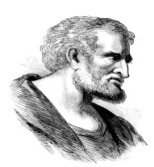
\includegraphics[width=1.773cm,height=1.931cm]{BUKU20INFORMASI202013-img1.jpg}
\end{figure}
\item Sampaikan ujud atau doa permohonan, lalu 
\item Bapa kami{\dots}{\dots}
\item Salam Maria{\dots}.(10x)
\item Kemuliaan{\dots}{\dots}
\item Terpujilah{\dots}{\dots}
\item Ya Yesus yang Baik{\dots}{\dots}.
\end{itemize}
(Setelah doa {\textquoteleft}Ya Yesus yang Baik{\textquoteright},
dilanjutkan dengan Misteri Kudus berikutnya dengan urutan doa yang sama
seperti di atas.)

\begin{enumerate}
\item Bacaan Injil (Bacaan: Epistola dan/atau Injil. Bacaan dapat
disesuaikan dengan tema peristiwa atau Maria sendiri)
\item Lagu Selingan 
\end{enumerate}
\begin{enumerate}
\item Dua Misteri Kudus (2x persepuluhan ke dua). Urutan doanya sama
seperti di atas.
\end{enumerate}
\begin{enumerate}
\item Ibadat Penutup
\end{enumerate}
\begin{itemize}
\item Doa Penutup dan mohon berkat Tuhan
\item Kolekte dan Lagu Penutup. Lagu Penutup selain untuk mengakhiri doa
Rosario juga mengiringi Kolekte.
\end{itemize}
Catatan: Doa Novena Roh Kudus akan dibuatkan Panduan Khusus.

\section[Tata cara persiapan dan pelaksanaan ujud \ \ \ misa/ibadat
pribadi]{Tata cara persiapan dan pelaksanaan ujud  misa/ibadat pribadi}
\begin{enumerate}
\item Misa/Ibadat yang dilaksanakan sendiri, tanpa melibatkan Lingkungan

\begin{enumerate}
\item Persiapan (dilaksanakan oleh umat ybs):

\begin{enumerate}
\item penentuan waktu
\item menghubungi Romo/petugas
\item persiapan koor (bila ada)
\item persiapan peralatan misa (bila ada misa)
\item pembuatan dan pengedaran undangan
\end{enumerate}
\item Pelaksanaan oleh umat bersangkutan:

\begin{enumerate}
\item pengaturan tempat
\item pengaturan Altar
\item penjemputan Romo/petugas (bila perlu)
\item pelaksaan misa/ibadat
\item penyerahan stipendium atau iura stolae untuk Romo
\end{enumerate}
\end{enumerate}
\end{enumerate}
\begin{enumerate}
\item Misa/Ibadat yang dilaksanakan oleh Lingkungan

\begin{enumerate}
\item Persiapan (oleh umat bersangkutan dan pengurus lingkungan):

\begin{enumerate}
\item penentuan waktu oleh umat
\item menghubungi Romo/petugas
\item persiapan koor (bila ada)
\item persiapan peralatan misa (bila ada misa)
\item pembuatan dan pengedaran undangan
\end{enumerate}
\item Pelaksanaan (oleh umat bersangkutan bersama dengan pengurus
lingkungan):

\begin{enumerate}
\item pengaturan tempat
\item pengaturan Altar
\item penjemputan Romo/petugas (bila perlu)
\item pelaksanaan misa/ibadat
\item penyerahan stipendium atau iura stolae untuk Romo
\item penggantian biaya hosti dan anggur
\end{enumerate}
\end{enumerate}
\end{enumerate}
Catatan:~Segala kegiatan doa/misa pribadi yang dipersiapkan dan
dilaksanakan sendiri (tanpa melibatkan Lingkungan) dengan melibatkan
banyak umat, keluarga bersangkutan wajib memberikan laporan kepada
Ketua Lingkungan untuk diteruskan ke Paroki.

\section[DOA{}-DOA]{DOA-DOA}
\subsection[DOA \ ANGELUS]{DOA  ANGELUS}
Maria diberi kabar oleh Malaikat TUHAN~ Maka Ia mengandung dari Roh
Kudus~ Salam Maria ...~  Aku ini hamba TUHAN~ Terjadilah padaku menurut
perkataanMU.~ Salam Maria ...~  Sabda sudah menjadi daging~ Dan tinggal
diantara kita~ Salam Maria~{\dots}..  Doakanlah kami, ya Santa Bunda
ALLAH~ Supaya kami dapat menikmati janji KRISTUS.~

Marilah berdoa: (hening sejenak)~ Ya Allah, karena kabar Malaikat kami
mengetahui~bahwa YESUS KRISTUS PutraMU menjadi manusia.~Curahkanlah
rahmatMU ke dalam hati kami,~supaya karena sengsara dan salibNYA,~kami
dibawa kepada kebangkitan yang mulia.~Sebab DIAlah TUHAN dan Pengantara
kami~.  Amin~

\subsection[DOA RATU SURGA (dalam Masa Paskah)]{DOA RATU SURGA (dalam
Masa Paskah)}
Ratu Surga bersukacitalah, alleluya,~ Sebab Ia yang sudi kau kandung,
alleluya,~

 Telah bangkit seperti disabdakan-Nya, alleluya!~ Doakanlah kami pada
Allah, alleluya!~

 Bersukacita dan bergembiralah, Perawan Maria, alleluya,~ sebab Tuhan
sungguh telah bangkit, Alleluya!~

Marilah berdoa (hening sejenak)~ Ya Allah,~ Engkau telah menggembirakan
dunia dengan kebangkitan PutraMu,~Tuhan kami Yesus Kristus.~Kami
mohon,~perkenankanlah kami bersukacita dalam kehidupan kekal bersama
BundaNya, Perawan Maria.~Demi Kristus, pengantara kami.~ Amin.

\subsection[SEJARAH DOA ANGELUS]{SEJARAH DOA ANGELUS}
Kita mengenal tradisi doa Angelus yang kita doakan pada jam 6 pagi, jam
12 siang dan jam 6 sore. Doa ini mempunyai 2 rumusan yakni rumusan
untuk dipakai pada masa Paskah dan rumusan untuk masa di luar Paskah.
Di Indonesia doa ini mulanya penggunaannya masih terbatas pada kalangan
kaum religius dan rohaniawan-rohaniwati. Akhir-akhir ini, doa Angelus
sudah semakin sering didoakan oleh umat awam.

\subsubsection[Arti]{Arti}
{\textquotedbl}Angelus{\textquotedbl} berarti
{\textquotedbl}Malaikat{\textquotedbl}.

\subsubsection[Mengapa dinamakan Doa Angelus?]{Mengapa dinamakan Doa
Angelus?}
Dinamakan Angelus karena kata ini merupakan kata pertama dari
{\textquotedbl}Maria diberi kabar oleh Malaikat{\textquotedbl} Yang
dalam bahasa latinnya adalah {\textquotedbl}Angelus domini nuntiavit
Mariae{\textquotedbl}

Doa Angelus sore hari dimulai pada abad ke-13 di Eropa. Oleh karena itu
doa Angelus sore hari ini yang pertama kali digunakan. Selanjutnya pada
pertengahan abad ke-14 barulah doa Angelus pagi hari digunakan di
seluruh Eropa. Doa Angelus pagi dan sore hari didoakan oleh para rahid
sebagai bagian dari doa pagi dan doa malam di biara-biara. Diawali
dengan doa Angelus kemudian dilanjutkan doa-doa harian para rahib
biara. Kemudian pada antara abad 14-15, barulah doa Angelus pada siang
hari muncul dan mulai didoakan.

\subsubsection[Tujuan Doa Angelus]{Tujuan Doa Angelus}
\begin{description}
\item[Doa Angelus jam 6 pagi: Menghormati kebangkitan Kristus.]

\end{description}
Yesus yang telah bangkit dan bersama Kristus kita memulai dari dengan
semangat kebangkitan.

Doa Angelus jam 12 siang: Menghormati sengsara Kristus.

Di tengah pekerjaan kita yang berat, kita senantiasa ingat Kristus yang
telah berkorban bagi kita.

Doa Angelus jam 6 sore: Menghormati Inkarnasi Allah menjadi manusia.

Pada saat kita beranjak untuk beristirahat, ingatlah bahwa Allah selalu
tinggal beserta kita.

\section[Doa masa Advent]{Doa masa Advent}
Ya Allah, Bapa yang Mahakudus kami bersyukur kehadirat-Mu, karena lewat
masa penantian ini Engkau menjanjikan Juruselamat yakni Yesus Kristus
Putra-Mu. Kedatangan-Nya dinubuatkan oleh para nabi dan dinantikan oleh
Perawan Maria dengan cinta mesra. Dialah Adam baru yang memulihkan
persahabatan kami dengan Dikau. Ia penolong yang lemah dan
menyelamatkan yang berdosa.

Ia membawa damai sejati bagi kami dan membuat semakin banyak orang
mengenal Engkau, dan berani melaksanakan kehendak-Mu. Ia datang sebagai
manusia biasa, untuk melaksanakan rencana-Mu dan membukakan jalan
keselamatan bagi kami. Pada akhir zaman ia akan datang lagi dengan
semarak dan mulia untuk menyatakan kebahagiaan yang kami nantikan.

Kami mohon kelimpahan rahmat-Mu, agar selama hidup di dunia ini kami
selalu siap siaga dan penuh harap menantikan kedatangan-Nya yang mulia,
agar pada saat Ia datang nanti, kami Kau perkenankan ikut berbahagia
bersama Dia dan seluruh umat kesayangan-Mu. Sebab Dialah Tuhan,
pengantara kami, kini dan sepanjang masa. (Amin)

\section[Doa masa Natal]{Doa masa Natal}
Allah Bapa disurga, kami memuji Engkau dan bersyukur kepada-Mu karena
sabda-Mu yang menjadi manusia dengan lahir ditengah-tengah kami. Ia
menjadi manusia lemah agar kami yang rapuh dan fana ini diurapi oleh
Daya ilahi yang Abadi.

Dengan kelahiran-Nya di dunia ini, Engkau yang tak dapat dilihat kini
kelihatan sebagai manusia seperti kami, dan cahaya keselamatan-Mu
bersinar ditengah kami, mengusir kegelapan yang menguasai kami.

Curahkanlah rahmat-Mu, agar kami yang kini merayakan misteri inkarnasi
berani menjadi pembawa damai bagi sesama, dan dengan demikian kami pun
menjadi sarana inkarnasi-Mu ditengah-tengah mereka. Dengan pengantaraan
Kristus, Tuhan kami, kini dan sepanjang masa (Amin).

\section[Doa masa PraPaskah]{Doa masa PraPaskah}
Allah Bapa yang maha kuasa, kami bersyukur kepada-Mu atas masa prapaskah
yang Kau anugerahkan kepada kami. Lewat masa prapaskah ini. Engkau
menginginkan kami untuk menyadari segala kebaikan-Mu. Selama masa
prapaskah ini Engkau melimpahkan rahmat untuk menyegarkan iman kami.

Engkau mengajak kami untuk bertobat, menyesali kekurangan dan dosa-dosa
kami. Engkau mendorong kami melepaskan diri dari belenggu nafsu yang
menyesatkan. Engkau mengajar kami untuk hidup sederhana, mensyukuri
segala anugerah-Mu, dan membantu orang-orang yang menderita. Selama
masa prapaskah ini Engkau membimbing para calon baptis yang akan
bersatu dengan kami melalui sakramen baptis. Sambil mendampingi mereka,
kamipun Kau ajak menyegarkan rahmat baptisan yang pernah kami terima
dari-Mu.

Semoga karena rahmat-MU, yang Kau limpahkah selama Masa Prapaskah ini,
kami semakin Suci, semakin bersatu dengan umat kesayangan-MU, dan
berani meneladani Yesus Putra-MU, yang rela menderita sengsara, wafat
dan bangkit untuk menyelamatkan kami. Sebab dialah Tuhan, pengantara
kami, kini dan sepanjang masa (Amin)

\section[Doa Paskah]{Doa Paskah}
Allah Bapa yang mahabaik, kami bersyukur kepada-Mu Karena Yesus Kristus
telah bangkit dari Kubur. Dengan kebangkitan-Nya. kau tumbuhkan
semangat dan harapan baru dalam hati kami; umat baru Kau ciptakan, dan
pintu surga Kaubuka bagi kami. Melalui kebangkitan-Nya kuasa Dosa kau
hancurkan, kami Kau damaikan dengan Dikau dan sesama, dan alam semesta
yang porak poranda Kaupugar kembali.

Dengan kenaikannya Ia merintis jalan kesurga, dan menyediakan tempat
bagi kami. Semoga karena Rahmat kebangkitan-Nya kami menjadi manusia
baru, yang penuh harapan, yang gigih melawan dosa dan kejahatan, yang
setia mengikuti kehendak-MU, dan tak gentar akan derita salib. Demi
Yesus Kristus, pengantara Kami, kini dan sepanjang masa. (Amin)

\section[Doa NOVENA Roh Kudus]{Doa NOVENA Roh Kudus}
Umat Kristen mempunyai kebiasaan mengadakan doa Novena Roh Kudus. Ini
dilaksanakan selama sembilan hari (novena = sembilan), mulai pada hari
sesudah kenaikan Tuhan Yesus ke surga dan berakhir pada hari Sabtu
menjelang Pentekosta. dalam doa ini umat Kristen memuji Tuhan yang
menjanjikan kedatangan Roh Kudus dan memohon rahmat Allah agar siap
menyambut kedatangan Roh Kudus. Doa ini juga bisa dilaksanakan pada
kesempatan lain yang cocok. Yang tersaji disini lebih dimaksudkan untuk
didoakan dalam kelompok; kalau didoakan secara pribadi, dapat
disesuaikan seperlunya.

Kalau Novena ini dipadukan dengan Perayaan Ekaristi, sesudah Mohon Tujuh
Karunia Roh Kudus menyusul Liturgi Ekaristi (persembahan, Doa syukur
Agung, dan seterusnya)

\subsection[Hari Pertama]{Hari Pertama}
Allah pokok keselamatan kami, karena kebangkitan Kristus kami lahir
kembali dalam pembabtisan dan menjalani hidup baru. Arahkanlah hati
kami kepada Kristus yang kini duduk di sebelah kanan-Mu. Semoga Roh-Mu
menjaga kami sampai Penyelamat kami datang dalam kemuliaan, sebab
Dialah Tuhan, Pengantara kami, kini dan sepanjang masa. Amin

Dilanjutkan dengan Rosario Roh Kudus ...

\subsection[Hari Kedua]{Hari Kedua}
Allah yang mahabijaksana, Putra-Mu menjanjikan Roh Kudus kepada para
rasul dan memenuhi janji itu sesudah Dia naik ke surga. Semoga kami pun
Kau anugrahi karunia Roh Kudus. Demi Yesus Kristus, Pengantara kami,
kini dan sepanjang masa. Amin

Dilanjutkan dengan Rosario Roh Kudus ...

\subsection[Hari Ketiga]{Hari Ketiga}
Allah, Penyelamat kami, kami percaya bahwa Kristus telah bersatu dengan
Dikau dalam keagungan. Semoga dalam Roh-Nya, Dia selalu menyertai kami
sampai akhir zaman, seperti yang dijanjikan-Nya. Sebab Dialah Tuhan
kami, kini dan sepanjang masa. Amin

Dilanjutkan dengan Rosario Roh Kudus ...

\subsection[Hari Keempat]{Hari Keempat}
Allah yang mahakudus, semoga kekuatan Roh-Mu turun atas kami, agar kami
mematuhi kehendak-Mu dengan setia dan mengamalkannya dalam cara hidup
kami. Demi Yesus Kristus, Tuhan kami, kini dan sepanjang masa. Amin

Dilanjutkan dengan Rosario Roh Kudus ...

\subsection[Hari Kelima]{Hari Kelima}
Allah yang mahakuasa dan mahakudus, semoga Roh Kudus turun atas kami dan
berdiam dalam diri kami, sehingga kami menjadi kenisah kemuliaan-Nya.
Demi Yesus Kristus, Tuhan kami, kini dan sepanjang masa. Amin

Dilanjutkan dengan Rosario Roh Kudus ...

\subsection[Hari Keenam]{Hari Keenam}
Allah yang mahaesa, Engkau telah menghimpun Gereja dalam Roh Kudus.
Semoga kami mengabdi kepada-Mu dengan ikhlas dan bersatu padu dalam
cinta. Demi Yesus Kristus, Tuhan kami, kini dan sepanjang masa. Amin

Dilanjutkan dengan Rosario Roh Kudus ...

\subsection[Hari Ketujuh]{Hari Ketujuh}
Allah yang mahakudus, curahkanlah Roh Kudus-Mu ke dalam diri kami,
sehingga kami dapat melaksanakan kehendak-Mu dan layak menjadi
milik-Mu. Demi Yesus Kristus, Tuhan kami, kini dan sepanjang masa. Amin

Dilanjutkan dengan Rosario Roh Kudus ...

\subsection[Hari Kedelapan]{Hari Kedelapan}
Allah sumber cahaya kekal, Engkau telah membukakan bagi kami jalan
menuju hidup kekal dengan memuliakan Putra-Mu dan mengutus Roh Kudus.
Semoga cinta bakti dan iman kami selalu bertambah. Demi Yesus Kristus,
Tuhan kami, kini dan sepanjang masa. Amin

Dilanjutkan dengan Rosario Roh Kudus ...

\subsection[Hari Kesembilan]{Hari Kesembilan}
Allah yang mahakuasa, kebangkitan Putra-Mu telah menumbuhkan hidup baru
dalam diri kami. Semoga karena bantuan Roh-Mu kami mewujudkan rahmat
kebangkitan dalam hidup kami sehari-hari. Demi Yesus Kristus, Tuhan
kami, kini dan sepanjang masa. Amin

Dilanjutkan dengan Rosario Roh Kudus ...

\section[ROSARIO ROH KUDUS]{ROSARIO ROH KUDUS}
Rosario Roh Kudus disusun pada tahun 1892 oleh seorang biarawan
Fransiskan Kapusin di Inggris sebagai sarana bagi umat beriman untuk
menghormati Roh Kudus. Doa ini kemudian memperoleh persetujuan
apostolik dari Paus Leo XIII pada tahun 1902. Rosario ini dimaksudkan
sebagai sarana untuk menghormati Roh Kudus, sama seperti Rosario Bunda
Maria di maksudkan para rahib Dominikan untuk menghormati Bunda Maria.

Rosario ini terdiri atas 5 kelompok manik-manik. Tiap kelompok terdiri
dari 7 manik. Sebelum dan sesudah tiap kelompok terdapat 2 butir manik
besar, sehingga seluruhnya ada 35 butir manik kecil dan 12 butir manik
besar. Sebagai tambahan, terdapat 3 manik kecil pada bagian permulaan.
Pada ketiga manik kecil ini dibuat tanda salib, lalu di daraskan doa
tobat dan himne datanglah Roh Pencipta.

Dalam tiap kelompok manik, diucapkan doa kemuliaan pada ketujuh manik
kecil, dan 1 doa Bapa Kami serta 1 Salam Maria pada kedua manik besar.
Pada 2 manik besar yang tersisa di bagian akhir, diucapkan Syahadat
Para Rasul (Aku percaya .....), doa Bapa Kami dan Salam Maria untuk
mendoakan Bapa Suci.

Pada doa ini terdapat 5 misteri: masing-masing misteri direnungkan pada
setiap kelompok manik-manik. Angka lima merupakan penghormatan atas
lima Luka Suci Yesus yang merupakan sumber rahmat yang dibagikan Roh
Kudus untuk seluruh umat manusia.

Secara berurutan, Rosario Roh Kudus di daraskan sebagai berikut:

Lagu Pembukaan

Tanda salib

Doa Tobat

Datanglah Roh Pencipta~ Datanglah hai Roh Pencipta~ Kunjungilah jiwa
kami semua~ Penuhilah dengan rahmat-Mu~hati kami ciptaan-Mu.

Gelar-Mu ialah penghibur~ Rahmat Allah yang mahaluhur~ Sumber Hidup, Api
Kasih~dan Pengurapan Ilahi.

Engkaulah sumber sapta karunia~ Jemari tangan Sang Ilahi.

Engkaulah janji sejati Allah Bapa~yang mempergandakan bahasa.

Terangilah akal budi kami,~ Curahkan cinta di setiap hati.

Segala kelemahan kami~semoga Kau lindungi dan Kau kuatkan.

Jauhkanlah semua musuh segera,~ Anugerahkanlah kedamaian jiwa,~ Dengan
Engkau sebagai penuntun kami~ Kejahatan tak{\textquotesingle}kan
mempengaruhi.

Perkenalkanlah kami kepada Bapa~ Ajarilah agar kami mengakui Putra~serta
Engkau, 

Roh dari Keduanya~yang kami imani dan puji selamanya.

Segala kemuliaan bagi Allah Bapa~dan bagi Sang Putra~yang telah bangkit
dari mati~serta bagi-Mu Roh Kudus pula~sepanjang segala abad.

Amin

Misteri Pertama:{\textquotedbl}Dari Roh Kuduslah Yesus dikandung Perawan
Maria.{\textquotedbl}~ (Renungan Luk1:35 )

Ujud khusus:~

Dengan tekun, mintalah bantuan dari Roh Ilahi serta perantaraan Bunda
Maria untuk mengikuti kebajikan-kebajikan Yesus Kristus, contohlah
segala kebajikan-Nya, sehingga kita dapat menjadi serupa dengan citra
Putra Allah.

Renungan dan doa pribadi ...~ Bapa Kami ...~ Salam Maria ...~ Kemuliaan
... (7x)

Misteri Kedua:{\textquotedbl}Roh Allah turun atas Yesus.{\textquotedbl}~
(Renungan Mat3:16 )

Ujud khusus:~

Peliharalah dengan penuh kesungguhan anugrah yang tak ternilai, rahmat
pengudusan yang dicurahkan dan ditanamkan dalam jiwa kita oleh Roh
Kudus pada saat pembaptisan. Peganglah dengan teguh janji baptis yang
telah kita ucapkan: tingkatkan iman, harapan dan cinta kasih melalui
tindakan nyata, serta hiduplah sebagai anak-anak Allah dan anggota
Gereja Allah yang sejati agar kelak kita dapat memperoleh warisan
surgawi.

Renungan dan doa pribadi ...~ Bapa Kami ...~ Salam Maria ...~ Kemuliaan
... (7x)

Misteri Ketiga:{\textquotedbl}Oleh Roh Kudus, Yesus dibimbing menuju
padang gurun untuk dicobai.{\textquotedbl}~ (Renungan Luk4:1-2)

Ujud khusus:~

Bersyukurlah selalu atas ketujuh karunia Roh Kudus yang dicurahkan pada
kita saat menerima Sakramen Penguatan: Roh kebijaksanaan, pengertian,
nasihat, keperkasaan, pengenalan akan Allah, kesalehan, dan rasa takut
akan Allah. Serahkan diri kita dengan setia kepada bimbingan Ilahi-Nya,
sehingga di atas segala godaan dan pencobaan hidup kita berlaku secara
perkasa sebagai seorang Kristen sejati dan prajurit Kristus yang
berani.

Renungan dan doa pribadi ...~ Bapa Kami ...~ Salam Maria ...~ Kemuliaan
... (7x)

Misteri Keempat :{\textquotedbl}Peranan Roh Kudus dalam
Gereja.{\textquotedbl}~ (Renungan Kis2:2 Kis2:4 Kis2:11 )

Ujud khusus:~

Bersyukurlah kepada Tuhan karena Ia menjadikan kita sebagai anggota
Gereja-Nya yang selalu dijiwai dan diarahkan oleh Roh Kudus, Roh yang
diturunkan ke dunia untuk tugas itu pada hari Pentekosta. Dengarlah dan
patuhilah Takhta Suci, wakil Roh Kudus yang tidak dapat salah, serta
Gereja, pilar dan dasar kebenaran. Junjunglah ajaran-ajarannya dan
belalah hak-haknya.

Renungan dan doa pribadi ...~ Bapa Kami ...~ Salam Maria ...~ Kemuliaan
... (7x)

Misteri Kelima:{\textquotedbl}Roh Kudus dalam jiwa-jiwa orang
beriman.{\textquotedbl}~ (Renungan 1Kor6:19 1Tes5:19 Ef4:30 )

Ujud khusus:~

Sadarilah keberadaan Roh Kudus dalam diri kita, peliharalah dengan
seksama kemurnian tubuh dan jiwa, ikutilah dengan setia bimbingan
Ilahi-Nya, sehingga kita dapat menghasilkan buah-buah Roh: kasih,
sukacita, damai sejahtera, kesabaran, kemurahan hati, kebaikan,
kesetiaan, kelemah lembutan, iman, kerendahan hati, penguasaan diri,
dan kemurnian.

Renungan dan doa pribadi ...~ Bapa Kami ...~ Salam Maria ...~ Kemuliaan
... (7x)~  Aku Percaya ...~ Bapa Kami ...~ Salam Maria ...

\begin{enumerate}
\item DAFTAR REMAJA dan MUDIKA LINGKUNGAN ST. PETRUS
\end{enumerate}
\begin{flushleft}
\tablehead{}
\begin{supertabular}{m{0.7cm}m{4.0090003cm}m{1.3149999cm}m{4.118cm}m{0.17599998cm}}
\centering No &
\centering Nama &
\centering Tahun Lahir &
\multicolumn{2}{m{4.494cm}}{\centering Orangtua}\\
 &
 &
 &
\centering Nama \& Alamat &
\centering\arraybslash Telpon\\
\centering 1 &
Y.V. Banesa Lanuardi &
\centering 1999 &
Andreas Winarso  Nanggulan &
HP.\\
\centering 2 &
Sisilia Widiastuti &
\centering 1999 &
Andreas Waldiman  Pugeran &
HP.\\
\centering 3 &
Emerentiana Krissanti Dewi Danudibroto &
\centering 1998 &
Lusia Krisni Prihartati Jl.P.Puger, Pugeran &
HP.085640438811\\
\centering 4 &
L. Dius Leonardo &
\centering 1998 &
Ign. Ludy Indra P.  Maguwo &
HP.\\
\centering 5 &
Eduardus Oldi Kristanto &
\centering 1998 &
Yohanes Suyanto  Sobomerter RT.06 RW 21 &
HP.085729157336

\\
\centering 6 &
R. Ade Kristian &
\centering 1997 &
Y. Eko Hananto  Nanggulan Rt.12 Rw. 18  &
HP:081392258790\\
\centering 7 &
B. Delphito Nugroho &
\centering 1997 &
Yohanes Suyanto  Sombomerten &
HP: 08562869037  Tlp: 0274-4333886\\
\centering 8 &
L. Tantri &
\centering 1997 &
Th. Banar Baharudin  Pugeran Gg. Bimo 21 RT.02 RW.64   &
HP: 085868421306\\
\centering 9 &
B. Wahyu Widodo &
\centering 1997 &
Aandreas Waldiman  Pugeran &
Hp.081568052255\\
\centering 10 &
S. Pratama Krisna Bayu Aji &
\centering 1997 &
P. S u r o y o  Pugeran Gg. Bawal RT.03 RW.09   &
HP:08122752803 Telp:0274-4333667\\
\centering 11 &
E. V. Sode Muda &
\centering 1996 &
A. Keso Muda  Pugeran Gg. Bima no.27 &
HP.08529243553\\
\centering 12 &
L. Veka Leanandra &
\centering 1996 &
I. Luddy Indra Purnama  Maguwo &
Tlp:0274-4333648 HP:08122700806\\
\centering 13 &
T. Edo Kristian &
\centering 1996 &
Y. Eko Hananto  Nanglan Rt.12 Rw. 18 &
HP:081392258790\\
\centering 14 &
V. Eko Cahyanto &
\centering 1995 &
C. Hendro Muryanto  Nanggulan &
HP: 081328032468\\
\centering 15 &
A. Adhi Wicaksana &
\centering 1995 &
Y. Budiman Susanto Karangnongko RT.09 RW.14   &
Telp.0274-4333578  Telp.0274-7471197 HP:08122942583\\
\centering 16 &
A. Merici Rianawati &
\centering 1995 &
H. Agus Marjuni  Nanggulan &
Telp:0274-487164 HP:081915536039\\
\centering No &
\centering Nama &
\centering Tahun Lahir &
\multicolumn{2}{m{4.494cm}}{\centering Orangtua}\\
 &
 &
 &
\centering Nama \& Alamat &
\centering\arraybslash Telpon\\
\centering 17 &
G. Meyta Dewi &
\centering 1995 &
B. Sami Rahardja  Pugeran RT.07 RW.65 &
Telp:0274-4333807 Hp:081578778777\\
\centering 18 &
M. Brenna Hernindia R. &
\centering 1995 &
A. Herry Purnomo  Karangnongko Jl.Nangka I/173A RT.09 RW.14  &
Telp.4333515 HP.08122762928 HP.081328200141\\
\centering 19 &
Paulina Iglia Lucia &
\centering 1995 &
Ign. Sandy  Pugeran RT.02 RW 64 &
HP.\\
\centering 20 &
R. Melati &
\centering 1994 &
Neo  S u r a d i  Pugeran &
Telp: 0274-556180  

HP: 081578115615\\
\centering 21 &
A. Tembang Saputra &
\centering 1994 &
A. Winarso  Nanggulan RT.11 RW 18 &
HP:0816675362

HP: 0816675362\\
\centering 22 &
V. Adhi Dharma &
\centering 1994 &
Y. Budiman Susanto Karangnongko RT.09 RW.14 &
Telp. 0274-4333578 Hp.08122942583\\
\centering 23 &
Ign. Stanley Andi Pradana &
\centering 1994 &
Y. Sugiyatno  Karangnongko RT.09 Rw 14 &
HP.\\
\centering 24 &
Y. Ferry Kurnia Dewi &
\centering 1993 &
Matheus Supangat  Nanggulan &
HP:081578043761,  HP: 0818277576\\
\centering 25 &
B. Laksmi Novita Sari &
\centering 1993 &
Y. Sugiyatno  Karangnongko RT.09 Rw 14 &
HP.:0811256059\\
\centering 26 &
A. Aditya Bimantara &
\centering 1993 &
Cornelius Supriadi  Pugeran &
Telp .0274-7497125  HP: 081328182141  

Telp: 0274-4333884\\
\centering 27 &
P. Sadewa Setyanto &
\centering 1993 &
Yohanes Suyanto  Sombomerten &
 HP: 08562869037  Tlp: 0274-4333886\\
\centering 28 &
D. Supri Astuti &
\centering 1992 &
A. Waldiman  Pugeran &
HP:081568052255\\
\centering 29 &
F. Agostinno Da Rosa &
\centering 1992 &
A. Dwi wahyuni  Sanggrahan &
HP: 081392704876\\
\centering 30 &
N. Novian Triatmojo &
\centering 1992 &
Y. Sugiyatno  Karangnongko RT.09 RW.14 &
HP.0811256059\\
\centering 31 &
B. Agusta Kristian &
\centering 1991 &
Y. Eko Hananto  Nanggulan RT.12 Rw.18   &
HP: 081392258790\\
\centering 32 &
C. Edlina Adiaty &
\centering 1991 &
Cornelius Supriadi  Pugeran &
Telp.0274-7497125  HP: 081328182141  Tlp: 4333884\\
\centering 33 &
P. Oktiva Rossari &
\centering 1990 &
A. Sujarwanto  Jl. P. Puger, Pugeran   &
HP: 08157955674  Telp: 4333577 \\
 &
\centering Nama &
\centering Tahun Lahir &
\multicolumn{2}{m{4.494cm}}{\centering Orangtua}\\
 &
 &
 &
\centering Nama \& Alamat &
\centering\arraybslash Telpon\\
\centering 34 &
M. Dwi Suryanto &
\centering 1989 &
I. S a m a n  Sanggrahan RT.03 RW.12   &
HP: 081578085478\\
\centering 35 &
Lusia Krisika Putri Wibowo &
\centering 1989 &
Lusia Krisni Prihartati  Jl.P.Puger, Pugeran &
HP.08559900326\\
\centering 36 &
F. Novka Kuaranita &
\centering 1988 &
A. Sujarwanto  Jl.P. Puger, Pugeran &
Hp.08157955674 Telp.0274-7475455\\
\centering 37 &
E. Alice Da Rosa &
\centering 1988 &
A. Dwi Wahyuni  Sanggrahan &
HP: 081392704876\\
\centering 38 &
A. Brian Rahardian Parahita &
\centering 1988 &
A.Y. Herry Purnomo  Karangnongko Jl.Nangka I/173A RT.09 RW.14  &
Telp.0274-4333515  HP: 08122762928  \\
\centering 39 &
A. Fenny Kurnianingsih &
\centering 1988 &
Ign. S a m a n  Sanggrahan RT.03 RW.12 &
HP.081578085478\\
\centering 40 &
F. Irwan Kristanto &
\centering 1987 &
Yakobus Lasiman  Sanggrahan &
HP.\\
\centering 41 &
M. Amarylis Illona Muda &
\centering 1987 &
A. Keso Muda  Pugeran Gg. Bima no.27   &
HP: 081392265997\\
\centering 42 &
Y. Bayu Rosanto &
\centering 1987 &
Y. Sugiyatno  Karangnongko   &
HP: 0811256059\\
\centering 43 &
D. Febrianto &
\centering 1987 &
Yoh. Suripto  Pugeran Gg. Nilam no.4   &
HP: 0817889303  Tlp: 0274-4333820\\
\centering 44 &
A. Satrio Adinugroho &
\centering 1986 &
Ignatia Sudarmini  Karangnongko 251 RT.6 RW.13   &
HP: 0811267658  Telp: 0274-4333604\\
\centering 45 &
S. Rio Setiawan &
\centering 1986 &
Y. Sugiyatno  Karangnongko RT.09 RW.14  &
HP.0811256059\\
\centering 46 &
B. Sukiwidhiyanto Prabowo &
\centering 1985 &
V. Ratnasih Anggreini Jl.Kembang A 24   &
Telp. 0274-488326 HP.08562907933\\
\centering 47 &
A. Leo Dilli Antoro &
\centering 1985 &
M. Supangat  Nanggulan &
HP:081578043761 HP:0818277576\\
\centering 48 &
Maria Anastasia Bare Lamakey &
\centering 1985 &
A. Lamakey  Pugeran Gg. Nilam no.6  &
Telp: 0274-4333684  HP: 081328034283\\
\centering 49 &
G. Fela Anggit Puspita Sari &
\centering 1985 &
Y. Sudarto  Nanggulan RT.04 RW.16 &
Telp. 0274-486955 HP.081328000523\\
\centering 50 &
G. Feli Anggit Puspita Sari &
\centering 1985 &
Y. Sudarto  Nanggulan RT.04 RW.16 &
Telp. 0274-486955 HP.081328000523\\
\centering 51 &
Maria Antonia Tona Lamakey &
\centering 1983 &
A. Lamakey  Pugeran Gg. Nilam no.6  &
Telp: 0274-4333684  HP: 081328034283\\
\end{supertabular}
\end{flushleft}
\end{document}
